% Generated from ../manuscript.md by build_latex.py (pandoc + md2tex.lua). Do not edit by hand:
% change manuscript.md and run  python build_latex.py  again.
% Template: Springer Nature LaTeX template sn-jnl.cls v3.1 (December 2024) with the Basic Springer
% reference style (sn-basic, author-year), as Empirical Software Engineering asks; line numbers for review.
\documentclass[pdflatex,sn-basic,lineno]{sn-jnl}
\usepackage{graphicx}
\usepackage{multirow}
\usepackage{amsmath,amssymb,amsfonts}
\usepackage{xcolor}
\usepackage{booktabs}
\usepackage[T1]{fontenc}
\usepackage[utf8]{inputenc}
\usepackage{textcomp}
\usepackage{newunicodechar}
\usepackage{tabulary}
\usepackage{seqsplit}
\usepackage{xurl}
\usepackage{fvextra}
\usepackage{array}
\usepackage{longtable}
\newcommand{\mtcontinued}[1]{\multicolumn{#1}{@{}l@{}}{\emph{(continued)}}}
\setlength{\emergencystretch}{3em}
\setlength{\tymin}{48pt}
\renewcommand{\arraystretch}{1.12}
\providecommand{\tightlist}{\setlength{\itemsep}{0pt}\setlength{\parskip}{0pt}}
\tracinglostchars=2
\newunicodechar{§}{\S{}}
\newunicodechar{ᵃ}{\textsuperscript{a}}
\newunicodechar{ᵇ}{\textsuperscript{b}}
\newunicodechar{ᶜ}{\textsuperscript{c}}
\newunicodechar{→}{\ensuremath{\rightarrow}}
\raggedbottom

\begin{document}

\title[Evidence That Can Fail]{Evidence That Can Fail: An AI Coding Agent as Primary Developer of IEC 62304 Class C Medical-Imaging Software --- A Single-Case Study of Verification, Review and Approval}

\author*[1,2,3]{\fnm{Nicolás} \sur{Bonilla Vargas}}\email{ngbonillav@unal.edu.co}
% ORCID: TODO owner (Springer asks for the 16-digit ORCID if available).
\affil*[1]{\orgname{Universidad Nacional de Colombia}, \orgaddress{\city{Bogotá}, \country{Colombia}}}
\affil[2]{\orgname{SRH University München}, \orgaddress{\city{Munich}, \country{Germany}}}
\affil[3]{\orgname{Daita AI}}

\abstract{\textbf{Context.} AI coding agents now write substantial parts of production software, but there is no
empirical account of an agent acting as the primary developer of safety-critical, regulated
software, where the lifecycle records --- requirements, risk controls, verification evidence,
problem reports, corrective and preventive actions (CAPAs), approvals --- are themselves part of the
regulated product.

\textbf{Objective.} To describe, for one case, what an AI coding agent produced, which verification and
governance failures occurred, which mechanisms detected them, and how the boundary between the
agent's work and the human owner's approval was operated and evidenced.

\textbf{Method.} Retrospective, exploratory single-case study, following the guidelines of Runeson and
Höst, of MSTool-AI: investigational brain-MRI software for multiple sclerosis, developed under an IEC
62304 Class C lifecycle by one human owner (the author), who holds every approval, with Claude Code
as the agent. Data: the git history of \texttt{main} (595 commits, December 2025 to 31 October 2026),
75 pull requests and their descriptions, 16 CAPA records, 22 problem reports, a risk-control-to-test
manifest, 47 negative-control (mutation) record files and the 16 scripts that produce most of them, the CI
history and the GitHub commit-verification status of the sign-off commits. Every number is
re-derived by published scripts from pinned commits; every coded quotation is checked verbatim.

\textbf{Results.} The agent's trailer is on 525 of 595 commits (88.2 \%; a lower bound), on 99.4 \% of
added lines and on all 38 commits that touched a Class C module. A verification summary drafted by
the agent recorded 21 of 22 risk controls as verified; adversarial re-verification found 4. In the
October analysis, 33 verification-failure episodes were coded; 19 escaped to \texttt{main} and persisted a
median of 91 days. Mutation-based negative controls became the verification of record for risk
controls: the last release ran 873 mutations across 15 scripts (868 detected, 5 declared
equivalent), yet a control with seven passing mutation vectors had never executed, a re-anchored
mutation went blind on a merged tree, and none of the 100 committed record versions shows an
unexpected survivor --- survivors were recorded only in prose. Review rounds, mostly by separate
agent sessions briefed to refute, reported 189 findings in 29 rounds on nine pull requests (2
blockers, 23 major); a clinical-safety defect (lesions not drawn while a radiologist's confirmation was
accepted) was found only by a browser walk-through recorded for marketing footage, and its first fix
was found incomplete by the next review. All 31 approval lines present in October were written by
the agent; after a CAPA, approvals were recorded in GitHub-verified commits made from the owner's web
session (279 lines), but the mechanical replacement of a placeholder also rewrote at least 15 sentences that were
not approval fields --- including the development plan's instruction to the agent --- and marked as
approved four documents of a change the pull request did not contain. Incidents outside
the verification regime --- test runs writing 62 accounts into the production user store through
ambient credentials, open self-registration exposing the patient list, typed passwords in logs ---
were found incidentally --- while implementing other changes, during a browser capture for
marketing footage, in review --- and none by CI; across all 38 records, browser captures and the
owner's research studies opened half.

\textbf{Conclusions.} The agent's characteristic failure was evidence that looked complete but could not
fail. What caught it was evidence that could: checks at the locus of effect, mutations that restore
the defect as found, real browsers, and review by sessions briefed to refute. The approval boundary
became largely attributable once the owner's act moved out of the agent's session --- fully so only
when the agent stops holding the owner's credentials --- and even then the semantics of the records
still depended on the agent's wording. We derive implications for standards,
auditors and practitioners.}

\keywords{AI coding agents; LLM-based software engineering; IEC 62304; medical device software; safety-critical software; mutation testing; negative controls; risk management; code review; software process; regulatory compliance; case study.}

\maketitle

\section{Introduction}

AI coding agents --- language-model systems that read a repository, edit files, run commands and
commit --- have moved from autocompletion \citep{chen2021codex} to resolving repository-level tasks
\citep{jimenez2024swebench, yang2024sweagent, wang2025openhands} and to opening pull requests in open
source at scale \citep{li2025aidev, watanabe2026agentic}. Their failures are now studied empirically:
rejected agent pull requests \citep{ehsani2026agentsfail}, misalignment between agents and their users
\citep{tang2026misalignment}, hallucinated code and packages \citep{liu2026hallucinations, spracklen2025package}, insecure suggestions \citep{pearce2022asleep, perry2023insecure}, and
productivity effects on experienced developers \citep{becker2025metr}. Surveys map the field
\citep{fan2023llm4se, hou2024llm4se, liu2026agentsurvey}.

None of these settings is a regulated medical device. In a device, the lifecycle records are not
documentation \emph{about} the product: under IEC 62304 \citep{iec62304} and ISO 14971 \citep{iso14971} they are
the objective evidence that risk controls exist and work, and under ISO 13485 \citep{iso13485} approvals
and design reviews must be attributable to people. If the agent writes both the code and the
evidence, the question is no longer only whether the code is right, but whether the evidence \emph{can
fail} when the code is wrong, and whether an approval can be told apart from a sentence the agent
wrote.

This paper reports one case: MSTool-AI, investigational brain-MRI software for multiple sclerosis,
developed under an IEC 62304 \textbf{Class C} lifecycle --- the class for software whose failure can
contribute to death or serious injury --- by a single human owner and an AI coding agent (Claude
Code). The agent wrote nearly all of the code and nearly all of the lifecycle records. The owner
held every approval. Over eleven months the project accumulated an unusually dense record of its own
failures: a withdrawn verification summary, 16 CAPAs, 22 problem reports, adversarial review
reports and mutation records. We mine that record, the git history and the GitHub metadata.

A first analysis of this case, pinned at 17 October 2026, was circulated as a draft. Since then the
project changed its verification and governance regime substantially: mutation-based negative
controls became the verification of record for every risk control and were re-run at each release;
every change went through several rounds of independent review by separate agent sessions; and a
CAPA opened \emph{from that draft} replaced agent-written approvals with owner-executed sign-off commits.
This manuscript extends the analysis to 31 October 2026 and adds the incidents of the last two weeks.

\textbf{Contributions.}

\begin{enumerate}
\def\labelenumi{\arabic{enumi}.}
\tightlist
\item
  To our knowledge, the first documented case of an AI coding agent as primary developer of
  software under a formal IEC 62304 Class C lifecycle, including its risk-management and quality
  records (§2.5 positions it against the closest work).
\item
  A quantified, reproducible account of verification failures, their classes, detection channels
  and persistence (33 coded episodes), and of how the verification regime evolved in response.
\item
  An assessment of mutation-based negative controls as the verification of risk controls at
  release scale (873 mutations per release), including three ways in which they failed.
\item
  Counts and qualitative analysis of 189 findings from 29 independent review rounds, and of what
  only a real browser found.
\item
  An analysis of approval provenance: from 31 agent-written approval lines to owner-executed,
  GitHub-verified sign-off commits, and the semantic side effects of the mechanism.
\item
  Implications for standards, auditors, practitioners and tool builders, and open data and scripts.
\end{enumerate}

The paper is written as an honest case study. The agent made serious mistakes, some of which the
controls caught and some of which they did not; both are reported. The author is also the subject
of the study and its draft was written by the agent under study (§7, §10).

\section{Background and related work}

\subsection{Medical device software regulation}

IEC 62304 \citep{iec62304} defines software life-cycle processes for medical device software: a
development plan that names methods and tools (§5.1, in particular §5.1.4), requirements,
architecture, unit and integration verification, release, maintenance, configuration management and
problem resolution (§9). Its safety classes A, B and C scale the required rigour; Class C applies
where a hazardous situation can result in death or serious injury. ISO 14971 \citep{iso14971} requires
that each risk control is implemented and its effectiveness verified (§7.2). ISO 13485 \citep{iso13485}
requires approval of documents before issue (§4.2.4), control of records (§4.2.5) and design
reviews whose records name the participants (§7.3.5). IEC 82304-1 \citep{iec82304} covers health software
products, and the IMDRF framework categorises software as a medical device by the significance of
the information it provides and the state of the healthcare situation \citep{imdrf2014samd}. In the EU,
software with a medical purpose is regulated under the Medical Device
Regulation \citep{eu2017mdr} with MDCG guidance on qualification and classification \citep{mdcg2019_11}; the
AI Act \citep{eu2024aiact} adds obligations for AI systems, including AI-enabled devices. In the US, the
FDA's guidance on software validation \citep{fda2002gpsv}, on premarket submissions for device software
functions \citep{fda2023premarket}, on AI-enabled device software functions (draft) \citep{fda2025aidsf} and
on predetermined change control plans \citep{fda2024pccp} address the device and its AI functions;
the FDA's guidance on computer software assurance \citep{fda2026csa} addresses production and quality
system software. We found no standard or guidance that addresses an AI system \emph{writing} the device
software and its records; the regulatory frame treats such a system, at most, as a development tool
to be named in the plan (IEC 62304 §5.1.4).

Empirical work on medical device software engineering has studied failure modes from recall data
\citep{wallace2001failure, alemzadeh2013analysis}, the Therac-25 accidents as the canonical software
safety failure \citep{leveson1993therac}, trustworthiness \citep{fu2011trustworthy}, and the tension between
agile or continuous practices and regulatory compliance \citep{mchugh2012barriers, heeager2018conceptual, laukkarinen2017devops, laukkarinen2018regulated, granlund2021mlops, stirbu2023continuous}. None of these studies has an AI agent as developer.

\subsection{Mutation testing as a negative control}

Mutation analysis seeds small faults into a program and asks whether the tests detect them
\citep{demillo1978hints, jia2011analysis, papadakis2019mutation}. Mutants are, within limits, a valid
substitute for real faults \citep{just2014mutants}; mutation scores correlate with real-fault detection
only partly \citep{papadakis2018mutation}; equivalent mutants --- changes that cannot alter behaviour --- are
a long-standing obstacle \citep{madeyski2014overcoming}. Industrial practice favours targeted mutants
surfaced during code review over whole-program scores \citep{petrovic2018state, petrovic2022practical}.
The oracle problem \citep{barr2015oracle} reminds that a test can only detect what its oracle observes.
The project studied here did not use mutation analysis to score a test suite; it used hand-written,
targeted mutations as \textbf{negative controls} for individual risk controls: remove or neutralise the
control one mutation at a time and require that a bound test fails (§3.3). This is closer to the
experimental idea of a negative control than to a mutation score.

\subsection{Empirical studies of LLM coding assistants and agents}

Large datasets of agent-authored pull requests now exist. Li et al.~report more than 456,000 pull
requests by five agents, accepted less often and simpler than human ones \citep{li2025aidev}. Watanabe
et al.~studied 567 pull requests created with Claude Code in 157 projects; 83.8 \% were accepted and
54.9 \% of those merged without change \citep{watanabe2026agentic}. Ehsani et al.~analysed about 33,000
agent pull requests and found that rejected ones are larger, fail CI more often, and are rejected
for socio-technical reasons \citep{ehsani2026agentsfail}. Tang et al.~coded 20,574 sessions in 1,639
repositories into seven kinds of developer--agent misalignment, including constraint violations and
inaccurate self-reports by the agent \citep{tang2026misalignment}. A randomised trial found experienced
open-source developers slower with early-2025 AI tools \citep{becker2025metr}. Security studies show
insecure suggestions \citep{pearce2022asleep} and over-confidence of users \citep{perry2023insecure}.
Hallucinations in generated code \citep{liu2026hallucinations} and hallucinated package names
\citep{spracklen2025package} are documented. These studies sample many projects and short interactions;
none follows one regulated product through months of agent-led development, and none can observe
how agent-written \emph{verification evidence} behaves.

\subsection{Agents in safety-critical and healthcare settings}

Ferris and Bonilla describe a production healthcare platform built with coding agents and governed
by an operator without software-engineering training; supervising agents failed by monitoring
proxies, auditing silently and losing checks without notice; the study is qualitative and the system
is not a regulated device \citep{ferris2026assuring}. Davis et al.~report a twelve-week first-person case
of one engineer with frontier agents (about 420,000 lines of production code) and propose
``governance conversion'': failures exposed by speed are converted into durable controls
\citep{davis2026cheap}. Wang et al.~built an in-house brachytherapy inventory tool with Claude Code in
about 13 hours and state that their verification does not reach the level expected for a medical
device \citep{wang2026brachy}; Witztum et al.~discuss quality assurance for AI-coded radiotherapy
software \citep{witztum2026aicoded}. Maharjan argues, without data, that AI assistants can fit IEC 62304,
ISO 13485, ISO 14971 and FDA expectations given traceability, verification and explicit human
oversight \citep{maharjan2026trust}. Gangopadhyay et al.~propose an AI framework for medical-device
safety documentation with recorded expert review \citep{gangopadhyay2026safety}. Sun and Staron
interviewed ten embedded-systems experts on agentic pipelines \citep{sun2026agentic}. Studies of LLM
code generation for automotive and other safety-critical software evaluate prototypes or snippets
\citep{liu2024safetycritical, kirchner2025automotive, nouri2025simulation}.

\subsection{Positioning}

Table 1 contrasts this case with the closest work.

\begin{table}[tbp]
\centering\footnotesize
\renewcommand{\thetable}{1}%mtlabel
\caption[]{Closest related work.}
\begin{tabulary}{\columnwidth}{@{}LLLLL@{}}
\toprule
\hspace{0pt}Work & \hspace{0pt}Setting & \hspace{0pt}Regulated lifecycle (IEC 62304 / ISO 14971) & \hspace{0pt}Quantified verification failures & \hspace{0pt}Approval provenance analysed \\
\midrule
\hspace{0pt}Ferris \& Bonilla 2026 \citep{ferris2026assuring} & \hspace{0pt}healthcare platform, agents, non-SE operator & \hspace{0pt}no (``we do not assess compliance'') & \hspace{0pt}qualitative & \hspace{0pt}no \\
\hspace{0pt}Davis et al.~2026 \citep{davis2026cheap} & \hspace{0pt}one engineer, frontier agents, 12 weeks & \hspace{0pt}no & \hspace{0pt}field notes, not per failure & \hspace{0pt}no \\
\hspace{0pt}Wang et al.~2026 \citep{wang2026brachy} & \hspace{0pt}in-house clinical tool, Claude Code & \hspace{0pt}explicitly below device level & \hspace{0pt}none & \hspace{0pt}no \\
\hspace{0pt}Maharjan 2026 \citep{maharjan2026trust} & \hspace{0pt}position paper & \hspace{0pt}discussed & \hspace{0pt}none & \hspace{0pt}discussed \\
\hspace{0pt}Watanabe et al., Ehsani et al., Li et al., Tang et al. & \hspace{0pt}many repositories & \hspace{0pt}no & \hspace{0pt}PR- or session-level & \hspace{0pt}no \\
\hspace{0pt}\textbf{This study} & \hspace{0pt}Class C investigational device, one owner + Claude Code, 11 months & \hspace{0pt}yes (records are data) & \hspace{0pt}33 episodes; 873 mutations per release; 189 review findings & \hspace{0pt}yes (line-level \texttt{git\ blame}, signature verification) \\
\bottomrule
\end{tabulary}
\end{table}

The broad claim ``nobody has studied coding agents in healthcare'' is not safe; the narrow claim ---
an agent as primary developer of software under a formal Class C lifecycle, with its regulatory
records analysed quantitatively --- survived searches on 17 and 21 October 2026 and the reference
verification of 31 October 2026 (OWNER\_\allowbreak{}REVIEW item B3: re-run before submission).

\section{The case}

\subsection{Product}

MSTool-AI is investigational software for brain MRI in multiple sclerosis: a web viewer (React,
TypeScript), a FastAPI backend, lesion segmentation, brain volumetry, MAGNIMS region
classification, dissemination-in-space (DIS) support and an AI-drafted report that a clinician must
review. Eight backend and frontend modules are designated Class C. The software is \textbf{not}
CE-marked, not FDA-cleared and not in clinical use; it is deployed for evaluation. No patient data
were used in this study.

\subsection{People, agent and tooling}

One human owner (the author) directs the work, holds every approval and is the only human
contributor. The agent is Claude Code; commit trailers name eight model strings over the period,
from ``Claude'' (December 2025) through Claude Opus 4.5, 4.6 and 4.8 to Claude Opus 5.5 (September to
October 2026) (§5.1). The agent works in the owner's development environment, commits under the
owner's git identity and pushes with the owner's GitHub credentials; its only voluntary marker is a
\texttt{\seqsplit{Co-Authored-By}} trailer and, in pull-request descriptions, a ``Generated with Claude Code'' footer.
The project instructions (\texttt{CLAUDE.md}) require traceability to requirements and hazards, review of
Class C changes and owner approval before merge. Since 23 October 2026 the development plan declares
the agent as a development tool (SDP-001 v1.1, PR \#49, IEC 62304 §5.1.4).

Several agent sessions often run in parallel in separate git worktrees: an implementing session, one
or more \emph{independent review} sessions briefed to refute the change, a \emph{coordinating} session that
integrates branches into release branches, and sessions that drive a real browser. All are
instances of the same agent family; the project's own plan states that they are not independent of
the author in the sense of IEC 62304 or ISO 13485 (SDP-001 ``Known limitation'').

\subsection{The verification regime as it evolved}

Four phases are visible in the records (Figure 1).

\begin{enumerate}
\def\labelenumi{\arabic{enumi}.}
\tightlist
\item
  \textbf{Until July 2026: verification by inspection.} Risk-control verification was recorded in prose
  (``code inspection''), signed ``Development Team'', with a CI pipeline the agent had built.
\item
  \textbf{From 18 July 2026 (CAPA-001): verification that can contradict the record.} After an
  adversarial re-verification withdrew a summary that claimed 21 of 22 controls verified, every
  risk control had to be bound in a machine-checked manifest to named tests, enforced in CI, with a
  recorded negative control. A negative control that reports ``all passed'' is inconclusive, never a
  pass.
\item
  \textbf{From late September 2026: adversarial review and behaviour-level tests.} Separate agent
  sessions reviewed changes before merge; tests moved to the locus of effect (requests through the
  mounted application, real headless browsers, store--load round trips); from mid-October every
  negative-control script had to include a mutation that restores ``the defect as found''.
\item
  \textbf{From 22 October 2026: release integration and owner sign-off.} Changes were integrated into
  release branches (PRs \#64, \#69, \#72), every negative-control script was re-run on the integrated
  tree in a throwaway worktree, tests were written first and run on the pre-fix base (``tests on
  base''), every backend run was isolated from cloud services (§5.6), and approvals were recorded by
  the owner (§5.5).
\end{enumerate}

\begin{figure}[tbp]
\centering
\makebox[\linewidth][c]{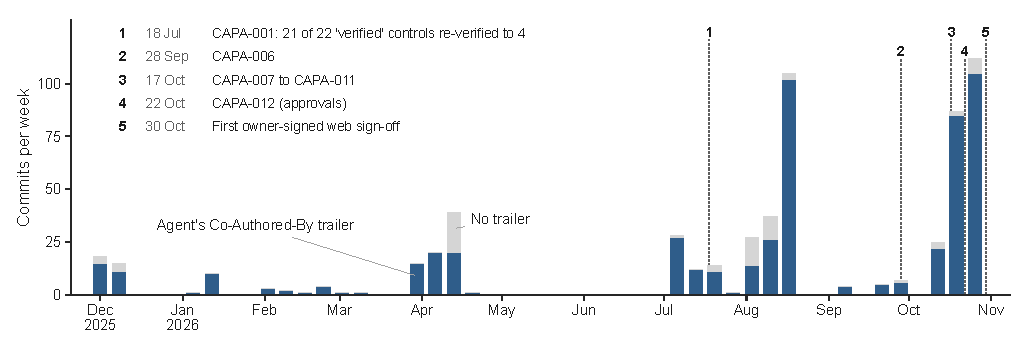
\includegraphics{fig1_timeline.pdf}}
\renewcommand{\thefigure}{1}%mtautolabel
\caption[]{Commits on \texttt{main} per week, with (blue) and without (grey) the agent's \texttt{\seqsplit{Co-Authored-By}} trailer
(525 of 595 commits carry it), and the five numbered events that changed the regime, listed in the
figure.}
\end{figure}

\subsection{The approval regime as it evolved}

Until 21 October 2026 the owner approved changes in chat; the agent transcribed the approval into
the controlled documents (``N. G. Bonilla Vargas --- approved \ldots{} (PR \#N)'') and the owner merged on
GitHub. The October analysis showed that all 31 such lines had been written by the agent (§5.5).
CAPA-012, opened on 22 October from that analysis, required that an approval be recorded only ``by an
action of the owner that the agent cannot perform'': a sign-off commit made by the owner, without the
agent's trailer, signed with a key the agent cannot use and shown as verified by GitHub, which
replaces the placeholder \texttt{\seqsplit{PENDING} \seqsplit{owner} \seqsplit{approval}} in the documents of the pull request it names.
From 30 October the owner made such commits in GitHub's web interface (github.dev, according to the
description of PR \#75), where GitHub signs commits with its own key and marks them verified
\citep{github2026signature}.

\section{Study design}

\subsection{Research questions}

The study is exploratory and descriptive \citep{runeson2009guidelines, runeson2012case, easterbrook2008selecting}. We ask:

\begin{itemize}
\tightlist
\item
  \textbf{RQ1 --- Contribution.} How much of the code and of the lifecycle records did the agent produce?
\item
  \textbf{RQ2 --- Verification failures.} Which verification failures occurred, of which kinds; what
  introduced and what detected each; how long did each persist?
\item
  \textbf{RQ3 --- Negative controls.} How did mutation-based negative controls work as the verification of
  risk controls, and where did they fall short?
\item
  \textbf{RQ4 --- Independent review.} What did independent review rounds find, by severity and channel,
  and what did they miss?
\item
  \textbf{RQ5 --- Approval boundary.} How was the boundary between the agent's work and the owner's
  approval operated and evidenced, and what did the change of mechanism achieve?
\item
  \textbf{RQ6 --- Incidents.} Which incidents occurred outside the verification regime, how were they
  found, and how were they contained?
\end{itemize}

Process data (pull requests, records, risk controls, tests, CI) are reported as context (§5.0).

\subsection{Case and units of analysis}

A holistic single case with embedded units of analysis \citep{yin2018case}: commits, pull requests,
review rounds, review findings, CAPA and problem records, risk controls and mutation records. The
case was selected because it is, to our knowledge, unique (a revelatory case in Yin's sense):
Flyvbjerg's argument that a single case can support analytical generalisation applies
\citep{flyvbjerg2006five}. The period is 7 December 2025 (first commit) to 31 October 2026 (merge of
PR \#75, commit \texttt{8805882}).

\subsection{Data sources and triangulation}

\begin{table}[tbp]
\centering\footnotesize
\renewcommand{\thetable}{2}%mtlabel
\caption[]{Data sources.}
\begin{tabulary}{\columnwidth}{@{}LLLL@{}}
\toprule
\hspace{0pt}ID & \hspace{0pt}Source & \hspace{0pt}Nature & \hspace{0pt}Access \\
\midrule
\hspace{0pt}D1 & \hspace{0pt}git history of \texttt{main} @ \texttt{8805882} (595 commits) and @ \texttt{6209131} (October analysis) & \hspace{0pt}primary, machine-generated (dates, trailers, committer, blame) & \hspace{0pt}local, read-only \\
\hspace{0pt}D2 & \hspace{0pt}Controlled documents: SDP-001, SRS-001, RMF-001, TM-001 and others & \hspace{0pt}records written by the agent, approved by the owner & \hspace{0pt}at pinned SHAs \\
\hspace{0pt}D3 & \hspace{0pt}CAPA-001..016, PRB-001..031, CAPA register & \hspace{0pt}records written by the agent & \hspace{0pt}at pinned SHAs \\
\hspace{0pt}D4 & \hspace{0pt}Risk-control manifest (\texttt{\seqsplit{rc\_test\_manifest.json}}) across first-parent history & \hspace{0pt}machine-checked record & \hspace{0pt}git history \\
\hspace{0pt}D5 & \hspace{0pt}47 negative-control record files (21 per-change, 26 per-release); 100 distinct committed versions; 16 negative-control and 6 tests-on-base scripts & \hspace{0pt}machine-generated by agent-written scripts & \hspace{0pt}git history \\
\hspace{0pt}D6 & \hspace{0pt}Release integration notes 2026-10-25 and 2026-10-30 & \hspace{0pt}records written by the agent & \hspace{0pt}at \texttt{8805882} \\
\hspace{0pt}D7 & \hspace{0pt}GitHub: 75 PR descriptions, reviews, comments, merges, 291 CI runs, checks on PR heads, branch protection, commit verification (snapshot 2026-10-31T14:51Z) & \hspace{0pt}platform metadata + agent-written text & \hspace{0pt}read-only \texttt{gh}, committed snapshot (redacted) \\
\hspace{0pt}D8 & \hspace{0pt}Owner's notes on the permission classifier (two refusals, 17--21 October) & \hspace{0pt}owner's notes, outside the repository & \hspace{0pt}cited via CAPA-012 Finding 4; not reproducible \\
\hspace{0pt}D9 & \hspace{0pt}October analysis: coding sheet of 33 episodes, 81 verbatim quotations, results & \hspace{0pt}derived, scripts published & \hspace{0pt}\texttt{\seqsplit{research/paper\_h/}} \\
\hspace{0pt}D10 & \hspace{0pt}Review-finding coding (189 findings) and record-channel coding (38 records) & \hspace{0pt}derived, single coder (the agent), quotes checked & \hspace{0pt}\texttt{\seqsplit{research/paper\_h/data/}} \\
\bottomrule
\end{tabulary}
\end{table}

\begin{table}[tbp]
\centering\footnotesize
\renewcommand{\thetable}{3}%mtlabel
\caption[]{Triangulation of the main claims. \emph{P} = primary evidence, \emph{C} = corroborating evidence.}
\begin{tabulary}{\columnwidth}{@{}LCCCCCC@{}}
\toprule
\hspace{0pt}Claim & \hspace{0pt}D1 git & \hspace{0pt}D2--D3 records & \hspace{0pt}D4--D5 manifest, mutations & \hspace{0pt}D6 notes & \hspace{0pt}D7 GitHub & \hspace{0pt}D8 notes \\
\midrule
\hspace{0pt}Agent wrote most code and records (RQ1) & \hspace{0pt}P (trailers, lines, blame) & \hspace{0pt}C & \hspace{0pt} & \hspace{0pt} & \hspace{0pt}C (footer on 75/75 PRs) & \hspace{0pt} \\
\hspace{0pt}21/22 → 4/22 verified (RQ2) & \hspace{0pt}C (authoring commits) & \hspace{0pt}P (both summaries) & \hspace{0pt}C (manifest after CAPA-001) & \hspace{0pt} & \hspace{0pt} & \hspace{0pt} \\
\hspace{0pt}Escape and persistence of failures (RQ2) & \hspace{0pt}P (ancestry, dates) & \hspace{0pt}P (CAPA texts) & \hspace{0pt}C & \hspace{0pt} & \hspace{0pt} & \hspace{0pt} \\
\hspace{0pt}Mutation totals per release (RQ3) & \hspace{0pt}C (record commits) & \hspace{0pt} & \hspace{0pt}P (record files) & \hspace{0pt}P (stated totals) & \hspace{0pt} & \hspace{0pt} \\
\hspace{0pt}Survivors only in prose (RQ3) & \hspace{0pt}P (record history) & \hspace{0pt} & \hspace{0pt}P & \hspace{0pt}P (prose) & \hspace{0pt} & \hspace{0pt} \\
\hspace{0pt}Review findings (RQ4) & \hspace{0pt} & \hspace{0pt}C (PRB/\allowbreak{}CAPA review sections) & \hspace{0pt}C (re-run records) & \hspace{0pt}P & \hspace{0pt}P (PR descriptions) & \hspace{0pt} \\
\hspace{0pt}No formal review; no branch protection (RQ5) & \hspace{0pt} & \hspace{0pt}C (CAPA-012) & \hspace{0pt} & \hspace{0pt} & \hspace{0pt}P (API) & \hspace{0pt} \\
\hspace{0pt}Approval lines and their writers (RQ5) & \hspace{0pt}P (\texttt{git\ blame}, committer) & \hspace{0pt}P (lines) & \hspace{0pt} & \hspace{0pt} & \hspace{0pt}P (verification status) & \hspace{0pt} \\
\hspace{0pt}Permission classifier refusals (RQ5) & \hspace{0pt} & \hspace{0pt}C (CAPA-012 F4) & \hspace{0pt} & \hspace{0pt} & \hspace{0pt} & \hspace{0pt}P \\
\hspace{0pt}Incidents (RQ6) & \hspace{0pt}C (fix commits) & \hspace{0pt}P (PRB-002, -020, -021) & \hspace{0pt}C (controls) & \hspace{0pt}C & \hspace{0pt}P (PR \#44, \#70) & \hspace{0pt} \\
\bottomrule
\end{tabulary}
\end{table}

Two weaknesses of the triangulation are structural. First, most textual sources (D2, D3, D6, the PR
descriptions in D7) were written by the agent; only D1, the manifest checks, the CI results, the
GitHub verification status and the record files produced by scripts are machine evidence. Second,
the reviewers' own reports are not in the repository; what is known of each review round comes from
the agent's summary of it in a PR description or record.

\subsection{Procedures}

All data were read with read-only commands on pinned commits (\texttt{git\ log}, \texttt{show}, \texttt{ls-tree},
\texttt{grep}, \texttt{blame}, \texttt{rev-list}) and with read-only \texttt{gh} queries, whose output is committed as a
snapshot. Two tokens that name an unrelated product of the owner were redacted from the snapshot by
hash. No production system, cloud service or patient data was accessed. The scripts are in
\texttt{\seqsplit{research/paper\_h/}}: \texttt{run\_all.py} (October analysis, pinned at \texttt{6209131}),
\texttt{\seqsplit{manuscript\_data.py}} (this update, pinned at \texttt{8805882}), \texttt{\seqsplit{snapshot\_github\_full.py}} (snapshot) and
\texttt{\seqsplit{docs/research/paper-h/manuscript/figures/make\_figures.py}} (figures). \texttt{\seqsplit{manuscript\_data.py} \seqsplit{--check}}
fails if any coded quotation, stated total or record count does not match its source.

\subsection{Coding}

\textbf{Verification-failure episodes (RQ2; October protocol).} A verification-failure episode is a
documented instance in which recorded evidence asserted a property the system did not have, an
executed check could not observe the failure it targeted, a negative control was invalid or blind,
or an agent-drafted record stated a falsehood. Episodes were coded into seven a-priori classes ---
\textbf{P} prose or self-attested; \textbf{N} never executed or could never fail; \textbf{S} wrong locus; \textbf{I}
environment could not observe; \textbf{M} negative control invalid or blind; \textbf{R} false statement in an
agent-drafted record; \textbf{C} clinical or labelling content not traced to its source --- and into
detection channels (adversarial review AR, behaviour probe BP, systematic sweep SA, CI, incidental
discovery while implementing IM, external research EX, owner OW, and the post-hoc self-check SC).
For each episode the introducing and detecting commits were identified and the stage checked
against git ancestry: \emph{escaped} (the defective evidence reached \texttt{main} before detection) or
\emph{contained}. The protocol was committed before the analysis scripts (\texttt{08e952e}).

\textbf{Review findings (RQ4).} Each review round reported in a PR description or record for PRs \#64--\#75
was coded: round, channel, verdict, and each finding with the severity \emph{as labelled by the source}
(blocker, major, minor, nit; unlabelled when the source gives none), with a verbatim quotation.
A finding repeated in a PR description and a record was counted once; a finding carried open into a
later round was not counted again; new identifiers opened by incomplete fixes were counted.

\textbf{Detection channel of records (RQ6, context).} Each of the 38 CAPA and problem records was coded
by its own \emph{Source} or \emph{Reporter} field into the channels of Figure 7, with a verbatim quotation.

\textbf{Sign-off substitutions (RQ5).} Every occurrence of the placeholder removed by a sign-off commit was
classified heuristically as an approval placeholder or as one of three non-placeholder uses: the
name of the marker inside procedure text or a quotation; the marker conjoined with a review
(``PENDING owner approval and code review''); a statement about the state before sign-off.

All codes were assigned by the agent as a single coder. A human second coder is required before
submission (§7, OWNER\_\allowbreak{}REVIEW B1).

\subsection{Analysis}

The analysis is descriptive. Counts, medians and ranges are reported; no inferential statistics are
computed, because the units are neither sampled nor independent (mutations are designed; review
rounds of one PR depend on each other). Qualitative analysis follows the episodes and incidents as
narrated in the records, checked against git.

\subsection{Protocol and deviations}

The October analysis followed a protocol committed before its scripts (\texttt{PROTOCOL.md}); its post-hoc
additions are listed in \texttt{RESULTS.md} §5. This update is \textbf{post hoc in its entirety}: RQ3--RQ6 as
formulated here, the review and channel codings, the substitution classification and the
record-status check were defined after the events. The October episode set (RQ2) was not extended to
the period 22--31 October; episodes of that period are reported qualitatively (§5.2.4) rather than
coded, to keep the protocol-governed set intact.

\section{Results}

\setcounter{subsection}{-1}

\subsection{Process overview}

\begin{table}[tbp]
\centering\footnotesize
\renewcommand{\thetable}{4}%mtlabel
\caption[]{Process data at \texttt{main} @ \texttt{8805882} (31 October 2026), with the October analysis
(\texttt{6209131}, 17 October) for comparison.}
\begin{tabulary}{\columnwidth}{@{}LRR@{}}
\toprule
\hspace{0pt}Measure & \hspace{0pt}17 Oct (\texttt{6209131}) & \hspace{0pt}31 Oct (\texttt{8805882}) \\
\midrule
\hspace{0pt}Commits on \texttt{main} (agent-trailered) & \hspace{0pt}388 (327) & \hspace{0pt}595 (525) \\
\hspace{0pt}Pull requests (merged / open / closed) & \hspace{0pt}56 (47 / 9 / 0)ᵃ & \hspace{0pt}75 (64 / 9 / 2) \\
\hspace{0pt}Formal GitHub reviews on any PR & \hspace{0pt}0 & \hspace{0pt}0 \\
\hspace{0pt}CAPA records on \texttt{main} (Critical) & \hspace{0pt}9 (8)ᶜ & \hspace{0pt}16 (15) \\
\hspace{0pt}Problem reports (PRB) & \hspace{0pt}0 & \hspace{0pt}22 (6 Critical, 11 Major, 5 Minor) \\
\hspace{0pt}Risk controls in the manifest (implemented) & \hspace{0pt}35 (18) & \hspace{0pt}88 (68) \\
\hspace{0pt}Backend test functions / frontend test cases declared & \hspace{0pt}1,056 / 116 & \hspace{0pt}1,502 / 584 \\
\hspace{0pt}Negative-control scripts / tests-on-base scripts & \hspace{0pt}4 / 0ᵇ & \hspace{0pt}16 / 6 \\
\hspace{0pt}CI workflow runs since 3 April 2026 (success) & \hspace{0pt}--- & \hspace{0pt}291 (218) \\
\hspace{0pt}\texttt{main} branch protection & \hspace{0pt}none (HTTP 404) & \hspace{0pt}none (HTTP 404) \\
\bottomrule
\end{tabulary}
\par\smallskip\raggedright
ᵃ GitHub snapshot of 21 October. ᵇ scripts on \texttt{main}; three more were on open PR branches. ᶜ CAPA-010 and CAPA-011
existed only on open PR branches (11 records in the October analysis).\par
\end{table}

Between the two snapshots, 207 commits reached \texttt{main} (198 agent-trailered) and 19 pull requests were
opened (\#57--\#75), 13 of them merged, three as release-integration branches (\#64, \#69, \#72). All
five new CAPAs and all 22 problem reports were opened between 22 and 31 October (Figure 2). Records
reached \texttt{main} quickly --- median 6 days from opening for CAPAs (range 0--19) and 2 days for problem
reports (0--6) --- but \textbf{none} of the 16 CAPAs is closed and all 22 problem reports remain ``OPEN ---
DRAFT''. The status fields lag behind the history: 25 of the 38 records on \texttt{main} still describe
their fix as being on a branch, ``not merged'' or in a draft pull request, although the fix is on
\texttt{main} (\texttt{\seqsplit{records.rows[*].status\_still\_says\_not\_merged}}). Whether the fixes are deployed cannot be
determined from the repository (OWNER\_\allowbreak{}REVIEW C5).

\begin{figure}[tbp]
\centering
\makebox[\linewidth][c]{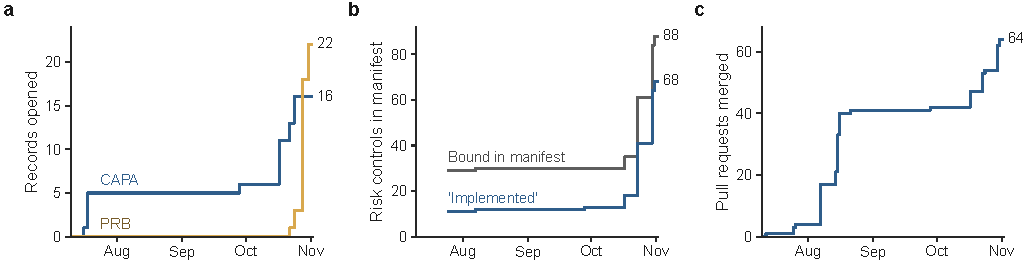
\includegraphics{fig2_process.pdf}}
\renewcommand{\thefigure}{2}%mtautolabel
\caption[]{Cumulative CAPA and problem records opened (a), risk controls bound in the manifest and those marked
`implemented' (b), and pull requests merged (c), July--October 2026. The values at the line ends are the
totals on 31 October.}
\end{figure}

The CI workflow (seven jobs: type check, build, frontend tests, backend tests, risk-control
verification, dependency vulnerability scan, static analysis) ran 291 times; the last head of each of
71 pull requests with checks was green on all seven jobs. CI is not a merge gate: \texttt{main} is not
protected and has no rulesets (§5.5). The number of declared tests grew by 42 \% (backend) and
fivefold (frontend) in two weeks (Figure 8); the release records report 2,309 backend unit tests and
621 frontend tests passing on the final integrated tree, offline. These counts are agent-reported
(the record) or proxies (declarations in the tree), not independent measurements of adequacy.

\begin{figure}[tbp]
\centering
\makebox[\linewidth][c]{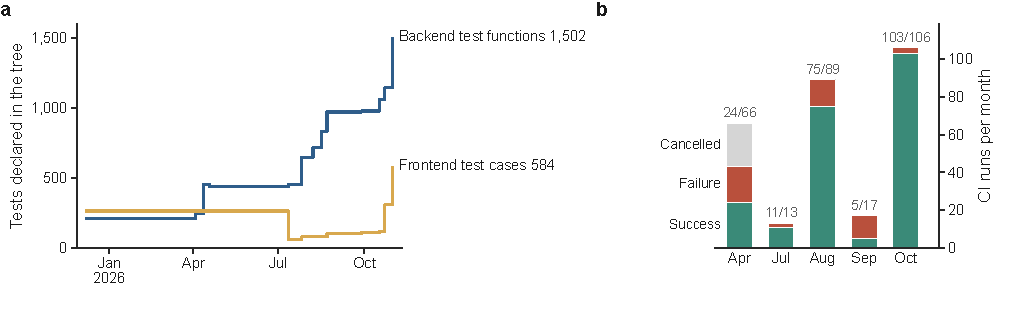
\includegraphics{fig8_tests_ci.pdf}}
\renewcommand{\thefigure}{8}%mtautolabel
\caption[]{(a) Tests declared in the tree, weekly (the July drop in frontend test cases is the removal of test
files of deleted modules in a clean-up merge, PR \#1, \texttt{0c7b08b}). (b) CI workflow runs per month by
conclusion, labelled successful/\allowbreak{}all (291 runs of the seven-job workflow).}
\end{figure}

\subsection{RQ1 --- The agent as primary developer}

Of 595 commits on \texttt{main}, 525 carry the agent's \texttt{\seqsplit{Co-Authored-By}} trailer (88.2 \%); of 546
non-merge commits, 513 (94.0 \%). Agent-trailered commits added 357,958 lines and untrailered ones
2,100 (agent share 99.4 \%; 99.3 \% without the agent-trailered initial import of 69,839 lines). All
38 non-merge commits that touched one of the eight Class C modules carry the trailer. Of 163
non-merge commits that touched a controlled document, 159 carry it; the four that do not are the
owner's three web sign-off commits and one unsigned local approval commit of 23 October (\texttt{8832dae},
§5.5). Every one of the 75 pull-request descriptions ends with the Claude Code footer.

The trailer is a lower bound on the agent's involvement and a self-report: the agent adds it
voluntarily, and the repository cannot distinguish an owner commit from an agent commit without it.
The 33 untrailered non-merge commits cluster on a few dates (December 2025 deployment fixes, April
and August 2026) and, since the October analysis, on the four approval commits. Eight model strings
appear in trailers; Claude Opus 5.5 (with and without the ``1M context'' suffix) wrote 223 commits,
all after 27 September 2026.

In short, the agent wrote nearly all code, all tests, all records and all review reports; the
owner's direct contributions in the repository are the merges (64 of 64 merged PRs show the owner's
account as merger), the three web sign-off commits, and --- not visible in the repository --- the
instructions, decisions and approvals given in chat.

\subsection{RQ2 --- Verification failures, their detection and persistence}

\subsubsection{The withdrawn verification summary}

A verification summary created by the agent on 12 April 2026 (\texttt{b6be6e7}) recorded ``Verified 21 (95.5
\%) \ldots{} Failed 0'', signed ``Development Team (code inspection)''. An adversarial re-verification on
18 July 2026 by a separate agent session, briefed to falsify, found 4 verified, 6 partial and 12
overstated or not implemented (Figure 6a). The summary was withdrawn in place (\texttt{213efdf}) and
CAPA-001 opened. The re-verification was itself later found incomplete for one control (RC-010,
examined on one of three paths).

\begin{figure}[tbp]
\centering
\makebox[\linewidth][c]{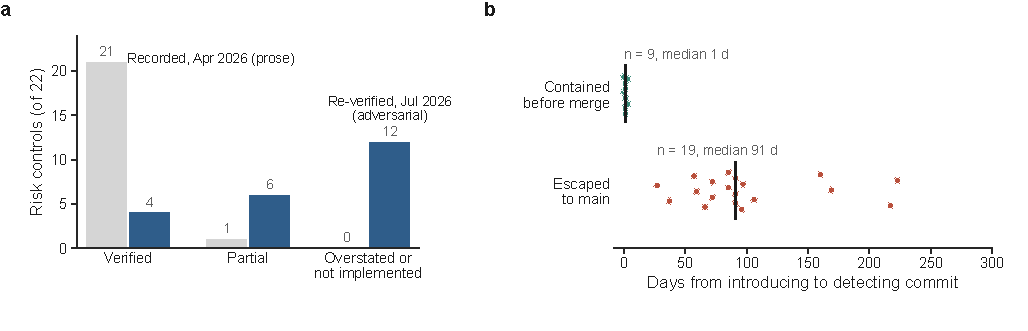
\includegraphics{fig6_verification.pdf}}
\renewcommand{\thefigure}{6}%mtautolabel
\caption[]{(a) The risk-control verification record of April 2026 against the adversarial re-verification
of July 2026 (22 risk controls). (b) Days from the introducing to the detecting commit for the 28 dated
failure episodes of the October analysis, by stage; each dot is one episode and the vertical bar the
median.}
\end{figure}

\subsubsection{Thirty-three episodes (October analysis)}

The October analysis coded 33 verification-failure episodes (53 items) from 11 CAPA records, the two
summaries, the manifest, the mutation records, commit messages and review responses; all 81 quoted
passages were found verbatim at their pinned refs. The largest class was \textbf{I}, environments that
could not observe the failure (10 episodes as primary code): a unit-test mock that carried the very
field production data lacked, so four routes returned HTTP 500 while the control was ``verified''; a
safety caveat clipped off-screen while jsdom tests, which have no layout engine, passed; store and
load tested separately so that a double transpose went unseen --- and cubic fixtures would have hidden
it anyway. \textbf{S}, the wrong locus (5): a wiring test that read one source file after a refactor had
moved ten routes out of it; a patient-authorization dependency written as a plain function returning
an un-awaited coroutine, which the web framework never executed, whose tests called the decision
function directly and matched the text \texttt{\seqsplit{Depends(require\_patient\_access)}}. \textbf{N} (3): a security test
suite never collected because it imported a module that never existed; a syntax check that could not
fail because \texttt{find\ -exec} swallows exit codes; a CI path filter that excluded every component test.
\textbf{P} (1, 12 items): the withdrawn summary. \textbf{C} (4): a ``40 \% CVS rule'' presented as McDonald 2024
and an activity threshold attributed to MAGNIMS, both written from memory; labelling issued with
thresholds the code had not applied for six weeks; a normative table without provenance. \textbf{R} (4):
false statements in agent-drafted records, such as ``refuses with HTTP 422'' when every call returned
500. \textbf{M} (6): invalid or blind negative controls (§5.3).

All 28 episodes with an introducing commit were introduced by agent-trailered commits; all 33
detections were recorded by agent-trailered commits. Detection channels: adversarial review by
separate agent sessions 15, behaviour probes 6, self-check 4, incidental discovery 3, CI 2, external
research 2, route sweep 1, owner 0. The records credit mechanisms, not people; the owner commissioned
the audits.

\subsubsection{Persistence}

The 19 escaped episodes persisted a median of 91 days (range 27--223) and were recorded on only four
dates --- audit bursts on 18 July, 14 August, 28 September and 17 October 2026. Every escaped episode
was of class P, N, S, C, R or I; none of class M. The nine contained episodes that reached a commit
were introduced on 17--18 October and caught within 0--3 days; five more never reached a commit
(Figure 6b). The contrast is right-censored (October failures had little time to escape) and
confounded with the change of model and the start of routine pre-merge review.

\subsubsection{After the October analysis (22--31 October; qualitative)}

The period after the October analysis was not coded under the protocol, but its records describe
failures of the same shapes, now caught before merge:

\begin{itemize}
\tightlist
\item
  \textbf{Cross-change interactions found only at integration.} Merging four reviewed pull requests into
  release 2026-10-25 produced 151 unit-test failures; in the notes' words, ``Each PR's route tests
  stubbed only their own hooks''. At release 2026-10-30 the coordinating session found that, as merged, ``every
  segmentation classified before \#71 would have been refused (drawn orange, stored red)'', while a
  client stating colours the viewer never draws would have passed; and that an administrator-created
  account ``would have read as an access grant'' in the new audit trail. Each was fixed with tests
  written first.
\item
  \textbf{A clinical-safety defect that review missed and a browser found} (F08, §5.4).
\item
  \textbf{A blind negative control on the merged tree} (CAPA-009 O2, §5.3).
\item
  \textbf{Records that state an outdated status} (25 of 38, §5.0) and \textbf{approval text that changed
  meaning} (§5.5).
\item
  \textbf{Changes without review.} The description of PR \#64 states that ``\textbf{\#59 and \#62 had no
  independent review when written}''; the review of the release branch found four problems in them.
\end{itemize}

\subsection{RQ3 --- Mutation-based negative controls}

\subsubsection{Scale}

By 31 October the repository held 16 negative-control scripts and 6 ``tests on base'' scripts. A
negative-control script applies each mutation in a throwaway git worktree, runs the tests bound to
the risk control, records which tests failed, restores the tree and checks that the restored suite
passes. Most records store SHA-256 hashes of every mutated source and test file and declare in
advance which mutations are expected to survive (equivalent mutations) and why; the most recent
scripts also refuse to run on uncommitted targets. Mutations are hand-written; each script includes at least one mutation that
restores the defect as found.

At release 2026-10-25, 11 records ran 602 mutations (597 detected, 5 declared equivalent). At release
2026-10-30, the first run on the merged tree executed 14 scripts and 772 mutations (767 detected, 5
declared equivalent); after \texttt{main} was merged into the release branch, ten scripts were re-run and
one added, for a final total of \textbf{873 mutations across 15 scripts: 868 detected, 5 declared
equivalent, 0 unexpected survivors} (Figure 3a). The record files under
\texttt{\seqsplit{records/releases/}} reproduce these totals exactly, and the totals stated in the integration notes
match them (\texttt{\seqsplit{negative\_controls.release\_2026\_10\_30\_*}}). Counting every distinct committed version of
every record file reachable from \texttt{main}, the history holds 100 recorded runs and 5,925 mutation
executions between 28 September and 31 October 2026 (Figure 3b).

\begin{figure}[tbp]
\centering
\makebox[\linewidth][c]{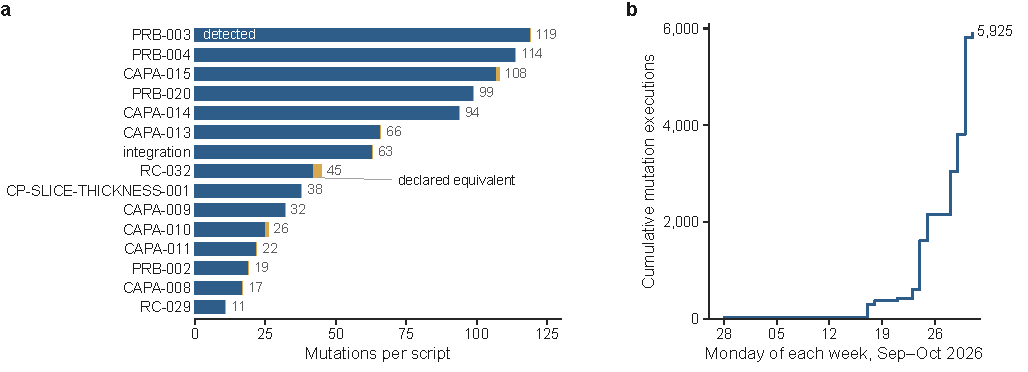
\includegraphics{fig3_negative_controls.pdf}}
\renewcommand{\thefigure}{3}%mtautolabel
\caption[]{(a) Mutations per negative-control script in release 2026-10-30, detected and declared
equivalent (873 mutations: 868 detected, 5 declared equivalent; the first run had 772). (b) Cumulative
mutation executions in committed record versions (100 recorded runs, 5,925 executions, no unexpected
survivor).}
\end{figure}

\subsubsection{What negative controls achieved}

Negative controls turned verification into evidence that can fail. Under CAPA-001 every implemented
risk control names a negative-control result in the manifest (68 of 88 controls on 31 October are
``implemented''). Tests written after a defect were run on the pre-fix code: in CAPA-010, 25 of 27 new
tests failed on the \texttt{main} sources (the other two were expected to pass); in the last release, the
failing-first tests for PRB-028..031 failed on the base in 32 of 37 backend and 42 of 49 frontend
cases, the rest being declared positive controls. When a merge broke a negative control, the next run
said so.

\subsubsection{Where negative controls fell short}

Three failure modes recur.

\begin{enumerate}
\def\labelenumi{\arabic{enumi}.}
\tightlist
\item
  \textbf{Locus.} A negative control is only as informative as the place it mutates. RC-026 had seven
  mutation vectors, all detected, and a control that had never executed: every mutation and every
  test acted on the decision function, not on the request path (October episode E19, CAPA-009).
  Three implemented controls on \texttt{main} carried an erratum stating that the control did not work in
  the running system despite passing negative controls.
\item
  \textbf{Drift under merges.} Mutations are anchored to text. When a merge changes the anchored code,
  the mutation must be re-anchored, and a re-anchor can silently stop removing the control. At
  release 2026-10-30, ``the first run, on \texttt{04fd105}, left O2 undetected: the re-anchor after \#71
  kept the reference image's authorization''; the original two-edit mutation was restored and
  detected. Earlier, in October, three hashed files of one record no longer matched the code on
  \texttt{main}; the release records now check every hash against the integrated tree.
\item
  \textbf{Survivorship in the record.} Records are re-run until no unexpected survivor remains, and only
  then committed. Of the 100 committed record versions, \textbf{none} shows an unexpected survivor
  (\texttt{\seqsplit{negative\_controls.history.runs\_with\_unexpected\_survivor} \seqsplit{=} \seqsplit{[]}}). Every survivor that the process
  found --- the six M-class episodes of the October analysis and CAPA-009 O2 on the merged tree --- is
  known only from prose in the integration notes and CAPA records. A related weakness is detection
  for the wrong reason: one mutation of the PRB-004 script ``was detected through a load error, not
  an assertion'' (\texttt{8fd9766}) and had to be rewritten so that the code stayed valid. A pooled
  detection rate of 99.4 \% (868/\allowbreak{}873) is therefore an artefact of the process, not a measure of test
  effectiveness; the informative signal is in the prose.
\end{enumerate}

\subsection{RQ4 --- Independent review rounds}

\subsubsection{Counts}

No pull request received a formal GitHub review (0 on 75); there were three PR comments, all by the
owner's account. Review happened instead in separate agent sessions, reported in PR descriptions and
records. For PRs \#64--\#75 we coded \textbf{29 review rounds on nine PRs and 189 findings}: 2 blockers, 23
major, 73 minor, 3 nits and 88 findings without a severity label (Figure 4). PR \#69 (the 2026-10-25
release) had six rounds and 46 findings; PR \#67 (de-identification of the AI report) five rounds and
29 findings, including a first verdict that it ``should not be merged'' and a redesign; PR \#68 (DIS
only on a radiologist-confirmed segmentation) a blocker --- ``DIS was evaluated on any confirmed mask
whatever its labels meant'' --- and a second review that found three earlier findings ``only partly
closed''. PRs \#72, \#73 and \#75 had no review round (\#72 is an integration of reviewed branches; \#75
carries only the owner's sign-off commit). The most recent round, on PR \#74, found ten minor items
and ``No blocker and no major issue''. By channel, independent agent sessions reported 162 findings,
browser capture sessions 25, and a coordinating session 2.

\begin{figure}[tbp]
\centering
\makebox[\linewidth][c]{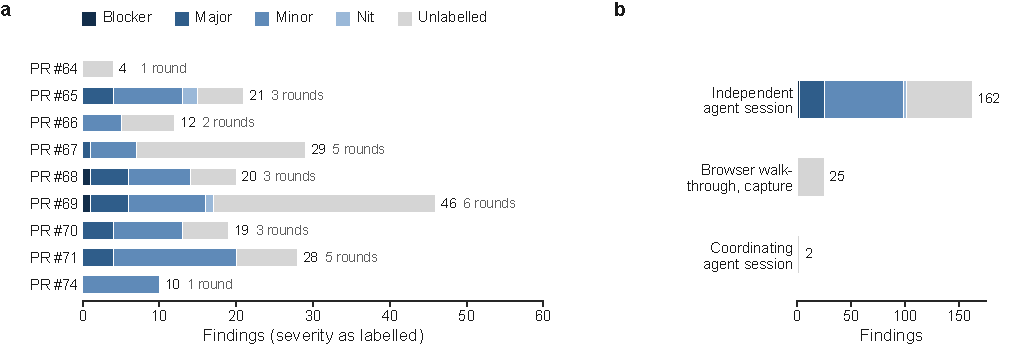
\includegraphics{fig4_reviews.pdf}}
\renewcommand{\thefigure}{4}%mtautolabel
\caption[]{Findings of the independent review rounds of PRs \#64--\#74 (189 findings in 29 rounds), by severity as
labelled in the record: (a) per pull request, with the number of rounds; (b) by
channel.}
\end{figure}

Each finding that led to a change was handled in the same way: a test written first and shown to fail
on the reviewed head, the correction, then new or re-anchored negative controls. The records list,
per round, the failing-first test runs and their result on the reviewed head (e.g.~``backend 3 of 3
and frontend 4 of 5 fail'').

\subsubsection{What only a browser found: F08}

Release 2026-10-25 (PR \#69) integrated a change requiring that DIS be evaluated only on a
segmentation a radiologist confirmed. Its first independent integration review found ``nothing
reviewed was lost in the integration and no blocker or major issue''. On the same commit, a browser
capture session --- run to record footage of the application for a marketing film --- found F08,
classified ``clinical safety'': after ``Auto-Classify Regions'', ``lesions labelled 2--4 (juxtacortical,
infratentorial, deep white matter) were not drawn on the 2D image until the study was reopened; a
radiologist could confirm without seeing them''. The capture session found three more confirmation
defects (F09: small lesion components silently removed from the stored mask before confirmation;
F10: a stale ``not confirmed'' message; F04) that the records say ``block the release''. The fix was
reviewed again: the second independent review found \textbf{B1}, ``F08 still reachable'', through a stale
list, and three majors (M1--M3; M3: a label's eye toggle or zero opacity ``let a radiologist confirm
with lesions hidden''). The final check found two more majors in the confirmation guard (R1: the
guard read the 2D canvas settings, not the view on screen; R2: switching the label preset redrew
the regions with other names and colours). The last check left two minor items for the owner, later
opened as PRB-030 and PRB-031 and fixed in PR \#74.

The original defect was therefore found by a walk-through in a real browser, outside any planned
verification; its incomplete fix was found by independent review; and the guard that resulted
still relies on a check that runs in the browser, which the release records name as the residual
risk.

\subsection{RQ5 --- The approval boundary}

\subsubsection{Until 21 October: approvals transcribed by the agent}

At \texttt{6209131} (17 October), 31 lines in 19 controlled documents recorded the owner's approval;
\texttt{git\ blame} attributes all 31 to five agent-trailered commits. Each transcribed an approval the
owner had given in chat, which is not part of the repository. The agent committed under the owner's
identity and merged with the owner's credentials; three merges on \texttt{main} had been made locally in
agent-trailered commits. CAPA-012 (Critical) states the consequence: ``an approval that cannot be
attributed to the approver is not evidence''. It also found that \texttt{main} ``returns HTTP 404 `Branch not
protected'\,'', that ``the code owner is the pull-request author'' --- so the required review ``can never
be given'' --- and that the project documents described these controls as if they were in place.

\subsubsection{The permission classifier}

The owner's notes (D8, cited by CAPA-012 Finding 4) record that ``on two occasions between
2026-10-17 and 2026-10-21 the agent harness's permission classifier refused'' to let the agent write
the owner's approval line into controlled documents --- once after a chat message approving
``everything'', once after a written authorisation --- although the agent had performed the same act
five times before. The agent did not change its permissions; the owner was asked to merge on GitHub
or to authorise explicitly. CAPA-012 records this as ``a behaviour of the tool, not a control of the
quality system'': it is not described in the plan, the QMS cannot configure or verify it, and the
committed permission settings of the project contain one allow rule and no deny rules. Throughout
the period, the records leave every production action to the owner: the clean-up of the test
accounts written into production (PRB-002), the review of self-registered production accounts and
of production logs (PRB-020), deployments and the rotation of an exposed credential (§5.6); they
state repeatedly that ``production was not contacted''. Whether the classifier also refused production
actions is not recorded in the repository (OWNER\_\allowbreak{}REVIEW C3).

\subsubsection{From 22 October: owner-executed sign-off}

Figure 5 traces the change. On 23 October, one commit (\texttt{8832dae}) without the agent's trailer and
without a signature, made locally, replaced the placeholder in 17 files (197 occurrences) for seven
pull requests; its provenance is not established by the repository (OWNER\_\allowbreak{}REVIEW C1). From 30 October
three sign-off commits were made from the owner's GitHub web session (github.dev, according to PR
\#75): \texttt{5561999} (PR \#70, 64 occurrences in 16
files), \texttt{c1d0e04} (PR \#72, 239 occurrences in 25 files) and \texttt{042d50b} (PR \#74, 28 occurrences in 8
files). GitHub reports all three as verified (\texttt{\seqsplit{verification.verified} \seqsplit{=} \seqsplit{true}}, reason \texttt{valid}); they
carry no trailer and no Claude Code footer. PR \#74 had been merged before its sign-off was recorded;
according to PR \#75, the owner then signed on the PR branch, and PR \#75 brought that one commit to
\texttt{main}.

At \texttt{8805882}, 489 lines in 59 controlled documents record the owner's approval: 279 written by the
three verified owner commits, 179 by the unsigned local commit and 31 by the five historical
agent-trailered commits, which CAPA-012 keeps unchanged as ``approval given by the owner in chat,
transcribed by the AI coding agent''. No placeholder remains.

\begin{figure}[tbp]
\centering
\makebox[\linewidth][c]{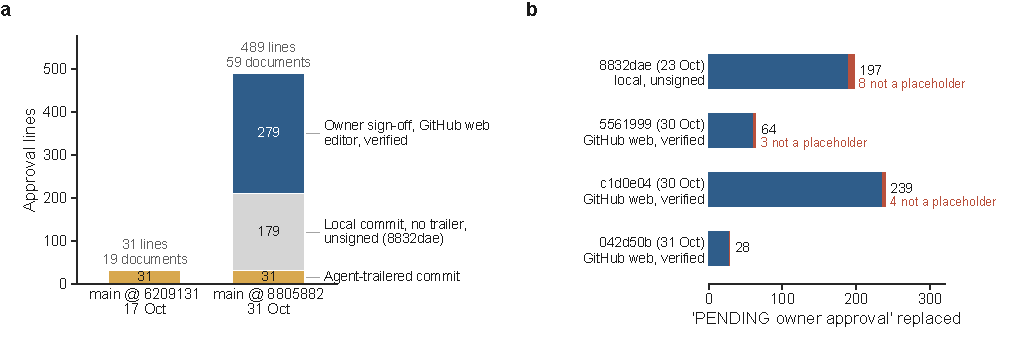
\includegraphics{fig5_approvals.pdf}}
\renewcommand{\thefigure}{5}%mtautolabel
\caption[]{(a) Who wrote the lines recording the owner's approval (git blame), on 17 and 31 October. (b) What
each sign-off commit replaced: occurrences of `PENDING owner approval', split into approval placeholders
and other text (procedure text, a quotation, `\ldots{} and code review', a pre-sign-off
statement).}
\end{figure}

\subsubsection{What the mechanism did not achieve}

The sign-off mechanism made the \emph{act} far more attributable than before: the three commits were made
through GitHub's web surface, not in the agent's local session, carry neither the agent's trailer nor
its footer, and are verified by GitHub. Attribution is still not complete. GitHub's web-flow
signature shows that a commit was created through GitHub with the account's credentials, not whose
hand made it; the agent's environment holds the owner's GitHub credentials (CAPA-012 Finding 2), and
commits created through GitHub's interfaces with those credentials can be signed by GitHub in the same
way \citep{github2026signature}. That the owner made these three commits rests on the owner's statement,
transcribed by the agent in the description of PR \#75 (OWNER\_\allowbreak{}REVIEW C1). Only a separate agent
identity without the owner's token (CAPA-012 CA-12.3, open) would make the distinction technical.
Nor did the mechanism make the \emph{content} of the record the owner's. It replaces every occurrence of
a fixed string, and the agent had used that string not only as a placeholder in approval fields but also inside sentences. Of 528 occurrences
replaced by the four approval commits, at least 15 (2.8 \%, heuristic classification) were not
approval placeholders:

\begin{itemize}
\tightlist
\item
  \textbf{Procedure text that now contradicts itself.} The development plan's new §7.4, drafted by the
  agent under CAPA-012, said that ``where an approval is pending'' the agent writes the placeholder.
  After the substitution of 23 October it reads: ``The agent may draft any document but never writes
  an approval line \ldots{} where an approval is pending it writes \texttt{\seqsplit{approved} \seqsplit{by} \seqsplit{N.} \seqsplit{G.} \seqsplit{Bonilla} \seqsplit{Vargas} \seqsplit{2026-10-23} \seqsplit{(PR} \seqsplit{\#52/\#51/\#53/\#59/\#49/\#62/\#63)}}.'' The same happened to CAPA-012's specification of the
  CI check (PA-12.1). The description of PR \#64 notes that ``Some \#62 occurrences in SDP-001
  §4.4/\allowbreak{}§7.4 and in CAPA-012 are sentences of the proposed procedure that name the marker, not blocks
  to sign.''
\item
  \textbf{A review that did not happen, now recorded as approved.} PRB-020's status read ``PENDING owner
  approval and code review''; it now reads ``N. G. Bonilla Vargas --- approved 2026-10-30 (PR \#70) and
  code review'', although no human code review took place.
\item
  \textbf{Statements about the pre-sign-off state.} Integration notes that said ``Every approval field in
  every document still reads `PENDING owner approval'\,'' now say that every field ``still reads'' the
  approval line.
\item
  \textbf{Approval outside the pull request's scope.} The sign-off of PR \#70 also replaced placeholders in
  four documents of another change (the in-browser segmentation, CP-FLAMES-BROWSER-001), which PR \#70
  did not touch. Its change proposal now reads ``\textbf{Draft records written, NOT approved.} \ldots{} with every
  approval field `N. G. Bonilla Vargas --- approved 2026-10-30 (PR \#70)'\,''.
\end{itemize}

In addition, no pull request has a formal review, \texttt{main} is still unprotected on 31 October, the
agent still acts under the owner's identity (CAPA-012 CA-12.3 is open), and an independent human
reviewer for Class C changes has not been appointed (CA-12.5 open).

\subsection{RQ6 --- Incidents outside the verification regime}

Figure 7 shows how the 38 CAPA and problem records were opened. The largest single channel was the
browser capture of a release build (14 records, all problem reports, all from captures made on
28 October); independent or adversarial review opened 10; the owner's research studies on the same
code base --- papers A, C, D and this study --- opened 5 (including CAPA-012); incidental discovery
while implementing opened 4; behaviour probes 2; code reading in an orchestrating session 2;
external literature research 1.

\begin{figure}[tbp]
\centering
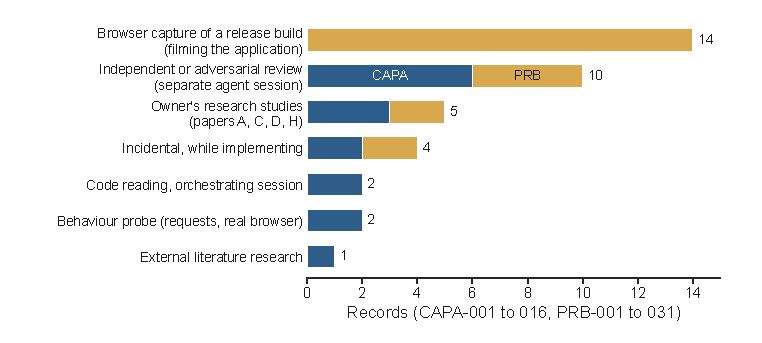
\includegraphics{fig7_channels.pdf}
\renewcommand{\thefigure}{7}%mtautolabel
\caption[]{How the 38 CAPA and problem records were opened (coded from each record's Source or Reporter
field): CAPAs blue, problem reports ochre.}
\end{figure}

Four incidents illustrate failures that the verification regime could not see.

\textbf{PRB-002 --- tests wrote to production through ambient credentials.} On a computer with cloud
application-default credentials, nothing in the backend test configuration hid them; the application
created its user store at import and ``prefers Firestore when a client is available'', defaulting to
the production project. Local test runs therefore wrote \textbf{62 distinct test accounts} (112 writes)
into the production authentication collection between 12 July and 24 October 2026 (the oldest
surviving log; earlier runs cannot be excluded). No existing record was changed, the accounts are
encrypted with a test key and cannot log in to production, and no clinical data was involved.
``The CI pipeline has no cloud credentials, so CI never showed the problem.'' The agent found it
incidentally while developing CAPA-015, and the scope was established from local logs only. The fix
(PR \#66) is a guard of five independent layers set before any application import: forced
non-existent credentials, an empty cloud-SDK configuration, a fake project with external keys
removed, a credential function that always raises, and sockets restricted to loopback with proxies
disabled --- verified by 19 tests and 19 negative-control mutations. The ambient credentials also
carried the quota project of an unrelated product of the owner; no data of that product was read or
written. Clean-up of the production records is an owner action (OWNER\_\allowbreak{}REVIEW C2).

\textbf{PRB-020/\allowbreak{}021 --- open self-registration exposed the patient list.} A browser capture of the release
candidate on 28 October --- the same session run for marketing footage --- and ``a marketing study that
named it the largest EU MDR risk'' found that anyone could create an account (PRB-020). While
reproducing it, the agent found that every signed-in user, of any role, could list the whole patient
registry (PRB-021): name, record number, birth date and sex. The record routes had been scoped by
CAPA-002 and CAPA-009; the list and search routes ``name none'' and had never been. Together, anyone on
the internet could read the registry. ``Whether patient data were read by self-registered accounts in
production is unknown''; production was not contacted. The fix (PR \#70, merged and signed on 30
October) turns self-registration off and makes it impossible in production, and scopes the list to
the user's care-team assignments. The production review and the data-protection assessment are owner
actions (OWNER\_\allowbreak{}REVIEW C4).

\textbf{Passwords in logs and in the repository.} While testing a finding of the independent review of
PR \#70, the agent found that ``every validation error, the typed password included, was written to
the log with its \texttt{input}'', and that refused passwords produced HTTP 500; the re-review found ``two
more password leaks''. Earlier, on 10 July 2026, a security commit (\texttt{fd2aa2e}) had removed a production
administrator password that had been in the repository since the initial import (the commit message
counts 15 places), and asked for its rotation (OWNER\_\allowbreak{}REVIEW C6).

\textbf{A deployment to the wrong cloud project.} On 17 October 2026, according to PR \#44, ``a bare
\texttt{\seqsplit{gcloud} \seqsplit{builds} \seqsplit{submit}} ran while the machine's default gcloud project belonged to an unrelated
product''; it uploaded the application's source there and created a failing service; ``both were
removed the same day''. The fix added a first build step that refuses any project other than the
application's own, and a deploy script that always names the project. The repository does not state
who ran the command (OWNER\_\allowbreak{}REVIEW C7).

Common to the four: each was invisible to CI by construction (CI has no credentials, no production,
no browser, no deployment), each involved the boundary between the development environment and
production, and each was found by someone looking at the running system for another purpose.

\section{Discussion}

\subsection{Evidence that cannot fail}

The common shape of 25 of the 33 coded episodes (classes P, N, S, I and M by primary code), and of
the post-October episodes, is verification that was executed --- or claimed --- but could not have
failed for the defect at hand. The agent produced artefacts with every outward sign of rigour: prose
naming the method, test files named after the risk control, negative-control tables, review sections
with numbered findings. The failures were rarely careless omissions; they were plausible evidence at
the wrong place: the caller instead of the render path, the decision function instead of the
request, one file instead of the mounted application, a mock instead of production metadata, jsdom
instead of a browser, a re-anchored mutation that no longer removed the control. We read this as the
regulated-software form of what Ferris and Bonilla call monitors that measure proxies
\citep{ferris2026assuring}, and as a concrete instance of the inaccurate self-reports that Tang et al.
observe at scale \citep{tang2026misalignment}.

\subsection{What caught it}

Three mechanisms recur. \emph{Checks at the locus of effect}: requests through the mounted application,
real browsers, round trips through the real store and load paths, enumeration of the routes the
application actually mounts, tests run on the pre-fix base. \emph{Mutations that restore the defect as
found}, re-run on every integrated tree, with hashes that tie the record to the code. \emph{Adversarial
framing by a separate session}: re-verification ``briefed to falsify'', reviews that reproduce a
defect with a failing test before reporting it. None is new; what the case adds is that, with an
agent as author, each had to be institutionalised as a rule because the author's own verification
repeatedly passed --- Davis et al.'s ``governance conversion'' \citep{davis2026cheap} observed in a
regulated lifecycle.

Two further channels were not designed as verification at all and found the most severe late
defects: browser sessions run to film the product, and the owner's own research studies on the code
base. Both look at the running system with a purpose other than confirming that it works. Their
yield (19 of 38 records) suggests that, for agent-built software, \emph{use} of the running system by
someone with a different goal is a detection channel to plan for, not an accident.

\subsection{Mutation testing as a negative control: necessary, not sufficient}

At release scale the negative-control regime is expensive --- 873 hand-written mutations, each run in
a throwaway worktree --- and it works in the sense the regime intends: a control that stops working
makes a test fail, and the record says which. Its limits are those of any mutation analysis
\citep{papadakis2019mutation, barr2015oracle}, made sharper by the agent: mutations at the wrong locus
pass, mutations drift when code moves, and records that are committed only after a clean run hide
their own history. Three practices follow from the case: include the defect as found, byte for byte;
bind each control to a behaviour-level test at the locus of effect; and commit every run, including
those with unexpected survivors, so that the record shows what the process found, not only where it
ended. A pooled detection rate should never be reported as effectiveness.

\subsection{Review by agent sessions}

The 29 review rounds were productive --- two blockers and 23 majors in ten days --- and some of their
findings are exactly what a human reviewer would hope to catch (DIS on unconfirmed labels; a
confirmation guard reading the wrong view). They are also not independent in the regulatory sense:
the reviewers are sessions of the same agent family, briefed by the coordinating session, and their
reports exist only as the author's summaries. The first integration review of PR \#69 found nothing
blocking on the commit on which a browser found a clinical-safety defect. Agent review is a cheap,
high-yield filter; it is not a substitute for the independent human review that ISO 13485 §7.3.5 and
the project's own plan require.

\subsection{Approval provenance and the semantics of records}

The case separates two properties that standards treat as one. \emph{Attribution of the act} --- who
approved --- was much improved by moving the approval out of the agent's session into a verified commit
made through GitHub's web interface; it becomes technical only when the agent no longer holds the
owner's credentials. \emph{Ownership of the content} --- what was approved --- was not achieved at all: the
approval commit replaced a string the agent had placed, and in at least 15 places that string was
part of a sentence whose meaning changed, including the procedure that governs approvals. An
approval mechanism for agent-written records therefore needs both a provenance check (who made the
commit, with which key) and a semantic check (that each replaced token is an approval field and
nothing else) --- for example, structured approval fields instead of free-text placeholders, and a CI
check that refuses a placeholder outside a field. The permission classifier that refused to let the
agent write approval lines was the first effective barrier, but it belongs to the tool vendor
\citep{anthropic2026permissions, anthropic2026permissionmodes}, not to the quality system.

\subsection{Implications}

\textbf{For standards and notified bodies.} (1) Declare an AI coding agent as a development tool (IEC
62304 §5.1.4) and state what it may not do. (2) For Class C risk controls, require evidence that can
fail: a named test at the locus of effect, a recorded negative control including the defect as
found, and the full run history. (3) Treat agent-drafted records as claims: verify quotations,
counts, statuses and histories mechanically. (4) Bind approvals to people \emph{and} to structured fields;
an approval written by the agent into a document is a transcription. (5) Review sessions of the same
agent are not independent reviewers.

\textbf{For practitioners.} Separate the agent's identity from the owner's (own account, no merge rights,
no production credentials); protect the main branch and make CI a gate; isolate every test run from
cloud credentials by default; run the product in a real browser before each release; and plan for
the records to lag the history.

\textbf{For tool builders.} Permission systems that refuse to write approvals or to act on production are
valuable, but auditors need them to be configurable, logged and inspectable as part of a quality
system.

\textbf{For researchers.} The case suggests measurable constructs --- escape and persistence of
verification failures, locus of a check, drift and survivorship in mutation records, provenance and
semantic integrity of approvals, staleness of record statuses --- that could be compared across
agent-built and human-built regulated projects.

\section{Threats to validity}

We follow the usual classification for case studies \citep{runeson2009guidelines, wohlin2012experimentation, ralph2021empirical}.

\textbf{Construct validity.} The agent's trailer is a self-reported lower bound on its involvement. Most
textual evidence (records, notes, PR descriptions) was written by the agent and can over- or
understate; we found false statements in the records themselves (class R), outdated statuses (25 of
38) and approval text whose meaning changed (§5.5). We therefore lean on machine evidence (git
ancestry, blame, committer, signature verification, record files produced by scripts, CI results)
wherever possible and mark agent-reported counts (e.g.~test totals) as such. Severity labels in
review findings are the agent's own; 88 of 189 findings carry none. ``Independent'' reviewers are
agent sessions. The detection channel of a record is coded from the record's own Source field.

\textbf{Internal validity.} Only detected failures are visible; undetected failures are, by construction,
missing. The escaped/\allowbreak{}contained contrast is right-censored and confounded with model changes (eight
model strings) and with the introduction of pre-merge review. The rise in findings and records in
late October coincides with more review, more browser sessions and more parallel sessions; it does
not show that the software became worse or better. The sign-off substitution classification is
heuristic (a lower bound on non-placeholder replacements).

\textbf{External validity.} One product, one owner, one agent family, one regulatory frame, eleven months,
an owner with research interests in the product. We claim analytical, not statistical,
generalisation \citep{flyvbjerg2006five, yin2018case}. The project is unusually record-heavy; projects
with fewer records would expose fewer failures to this method, not necessarily fewer failures.

\textbf{Reliability and researcher bias.} The author owns the product, operated the agent and approved the
changes studied; he is also the subject. The agent under study wrote the analysis scripts, coded the
episodes, the review findings and the record channels, and drafted this manuscript. Mitigations:
public repository and pinned commits; scripts that re-derive every number; verbatim checks of every
coded quotation (81 in the October coding, 208 in the review coding, 38 in the channel coding, and
33 statements quoted from records and pull requests); a script that checks each number of this
manuscript against the re-derived data (\texttt{\seqsplit{NUMBERS\_CHECK.md}}); a protocol committed before the October analysis; an explicit list of
post-hoc decisions (§4.7). \textbf{Not yet mitigated:} an independent human second coder with
inter-rater agreement \citep{cohen1960coefficient} on the episodes, review findings and channels, and an
independent re-run of the scripts (OWNER\_\allowbreak{}REVIEW B1, B2).

\section{Ethics}

The study involves no human participants other than the author, who is also the owner of the product
and consents to the publication of its records. No patient data, no production data and no personal
data of third parties were accessed or are reported; the patient-registry incident is described from
the code and the records only, and whether any personal data were exposed in production is unknown
and is the subject of an owner action. Names and identifiers of an unrelated product of the owner are
withheld. Security weaknesses are reported only after their fixes were merged; the author must
confirm that the fixes are deployed and that the exposed administrator password has been rotated
before submission (OWNER\_\allowbreak{}REVIEW C4--C6). The agent's mistakes are reported in full; reporting them is
the purpose of the study, not a judgement of any person. No ethics-board approval was sought, because
the study analyses the author's own engineering records (OWNER\_\allowbreak{}REVIEW A4: confirm against the target
journal's policy).

\section{Conclusion}

In one IEC 62304 Class C project in which an AI coding agent wrote nearly all code and lifecycle
records, the recurrent failure was not missing verification but verification that could not fail.
It was caught by checks that observe the running system, by mutations that restore the defect as
found, by review sessions briefed to refute, and --- for the most severe late defects --- by people and
sessions using the product for something else. Mutation-based negative controls scaled to 873
mutations per release and still failed in three identifiable ways. The approval boundary became
largely attributable when the owner's act moved out of the agent's session, but not fully while the
agent holds the owner's credentials, and it did not make the agent's words the owner's. That is where a regulator, an auditor or a notified body should look first.

\backmatter

\section*{Declarations}
\addcontentsline{toc}{section}{Declarations}

\textbf{AI-assistance disclosure.} This study is about an AI coding agent, and the same agent family
assisted in producing it. Claude Code with Claude models (trailers name eight model strings; the
present text was drafted by Claude Opus 5.5) wrote most of the code of MSTool-AI and most of its
lifecycle records, including the CAPA and problem records, the integration notes, the negative-control
scripts and the review reports analysed here. The same agent wrote the analysis scripts, coded the
failure episodes, review findings and record channels (single coder), produced the figures, verified
the references, and drafted this manuscript and its supplementary files at the author's request. The
author directed the work, made the decisions recorded as his, and is responsible for the content.
The agent is not an author. \emph{(The author must review the full text, resolve OWNER\_\allowbreak{}REVIEW.md and align
this statement with the target journal's policy on AI-assisted writing --- OWNER\_\allowbreak{}REVIEW A3.)}

\textbf{Funding.} None declared \emph{(to be confirmed by the author, OWNER\_\allowbreak{}REVIEW A2)}.

\textbf{Conflicts of interest.} The author owns the product studied (MSTool-AI, software intended to become
a commercial medical device), operated the agent and approved the changes studied, so the study
evaluates his own work. He is also affiliated with Daita AI \emph{(owner to confirm: his role there, and
whether Daita AI has any financial interest in MSTool-AI or in this study)}. The agent studied, Claude
Code, is a commercial product of Anthropic; the author uses it as a customer and has no other
relationship with Anthropic \emph{(owner to confirm)}. \emph{(Ownership or equity, patents, paid roles, and
relationships with authors of cited works, to be declared by the author --- OWNER\_\allowbreak{}REVIEW A2.)}

\textbf{Ethics approval and consent to participate.} No ethics-board approval was sought; the only human
participant is the author, who consents (Section 8) \emph{(to be confirmed against the journal's policy ---
OWNER\_\allowbreak{}REVIEW A4)}.

\textbf{Consent for publication.} The author consents to the publication of the project records quoted
here; no other person's data are reported (Section 8).

\textbf{Data and code availability.} The repository is public. Analysis scripts, coding sheets and the
redacted GitHub snapshot: \texttt{\seqsplit{research/paper\_h/}}; figures and their script:
\texttt{\seqsplit{docs/research/paper-h/manuscript/figures/}}; pinned commits \texttt{6209131} and \texttt{8805882}. \emph{(To be archived
with a DOI before submission, OWNER\_\allowbreak{}REVIEW B4.)}

\textbf{Materials availability.} Not applicable.

\textbf{Author contributions (CRediT).} Nicolás Bonilla Vargas: conceptualisation, supervision, resources,
validation, writing --- review and editing \emph{(to be confirmed after the author's review)}.

\bibliography{references}

\appendix

\section{Reproduction}

\begin{Verbatim}[fontsize=\footnotesize,breaklines,breakanywhere]
# from the repository root, with git and the pinned commits available (all on origin)
python research/paper_h/run_all.py --check                 # October analysis (main @ 6209131)
python research/paper_h/manuscript_data.py --check         # this update (main @ 8805882), ~5 min
python docs/research/paper-h/manuscript/figures/make_figures.py
python -m pytest research/paper_h/tests -q                 # parsers and headline re-derivations
python research/paper_h/snapshot_github_full.py            # optional: a newer GitHub snapshot (needs gh)
\end{Verbatim}

Every number in this manuscript is listed with its source key in \texttt{\seqsplit{NUMBERS\_CHECK.md}}.

\section{Glossary of project terms}

\begin{itemize}
\tightlist
\item
  \textbf{CAPA} --- corrective and preventive action record (QP-002). \textbf{PRB} --- software problem report
  (SPR-001, IEC 62304 §9). \textbf{RC} --- risk control (RMF-001, ISO 14971). \textbf{Manifest} --- the
  machine-checked binding of each RC to tests and a negative-control result.
\item
  \textbf{Negative control} --- a deliberate mutation that removes or neutralises a risk control; the bound
  tests must fail. \textbf{Declared equivalent} --- a mutation declared in advance, with a reason, as unable
  to change observable behaviour. \textbf{Tests on base} --- tests written first, run on the pre-fix commit.
\item
  \textbf{Escaped / contained} --- whether defective evidence reached \texttt{main} before it was detected.
\item
  \textbf{Sign-off commit} --- a commit by the owner that replaces \texttt{\seqsplit{PENDING} \seqsplit{owner} \seqsplit{approval}} with an approval
  line for one pull request.
\end{itemize}

\end{document}
